\section{绪论}

\subsection{选题背景}
互联网技术的蓬勃发展在很大程度上给人们的生活带来了越来越多的便利,人们在逐渐适应网络这样的平台的同时,也更倾向于甚至依赖在网络平台上完成生活中的各种事情,可以说,网络对于人们的重要性已经几乎等同于空气、水和食物。按照网络平台的功能来划分,门户网站(新浪、搜狐等)是新闻实事评论发布的主要渠道,社交网站(微博、人人等)是人们分享个人想法和心情的首选,博客系统(新浪博客、百度空间等)是人们发表和传达思想和经验的主要平台,以及一些新新涌现的图片和视频等多媒体资源分享平台(优酷土豆、POCO等)大大丰富了人们的娱乐生活。此外,鉴于国内发达的物流行业,各大电子商务平台(淘宝、京东等)也使得不用出门就能购物成为了现实。按照网络平台资源的载体来划分,包括文本、图片、音乐和视频几大类,其中文本无疑是整个互联网资源的主体,无论是传统的新闻、博客、评论、说明,还是新新发展的弹幕视频网站(Acfun\footnote{http://www.acfun.tv/}、Bilibili\footnote{http://www.bilibili.com/}等),都是由很多文本信息组成的。按照网络平台的用户参与角度来划分,可以将用户角色分为两种:信息发布者和信息获取者。以程序员为例,当他需要学习一项新技术时,往往会通过搜索引擎寻找一些与该技术相关的教学经验文章,从而使自己尽快掌握该项技术。等对该技术数量掌握之后,往往又会通过写技术博客的方式记录下他的学习历程和使用中的经验之谈,以供他人参考。同时,该用户还肯定拥有其他多个兴趣爱好,比如他可以与网上其他用户分享旅游游记、摄影作品等等。

虽然这些网站系统在功能上、信息载体上或是用户参与方式上都截然不同,但是宏观来看他们都存在一个共同的问题:信息孤岛现象。如图\ref{fig:problem}所示,当这些网站发展越来越多之时,各个网站之间信息不流通的问题也日渐明显,每个网站独立发展,出于安全性等方面的考虑,其资源和用户的数据并不能实现跨平台共享,从而使得每个网站成为一座座信息孤岛。

\begin{figure}
\centering
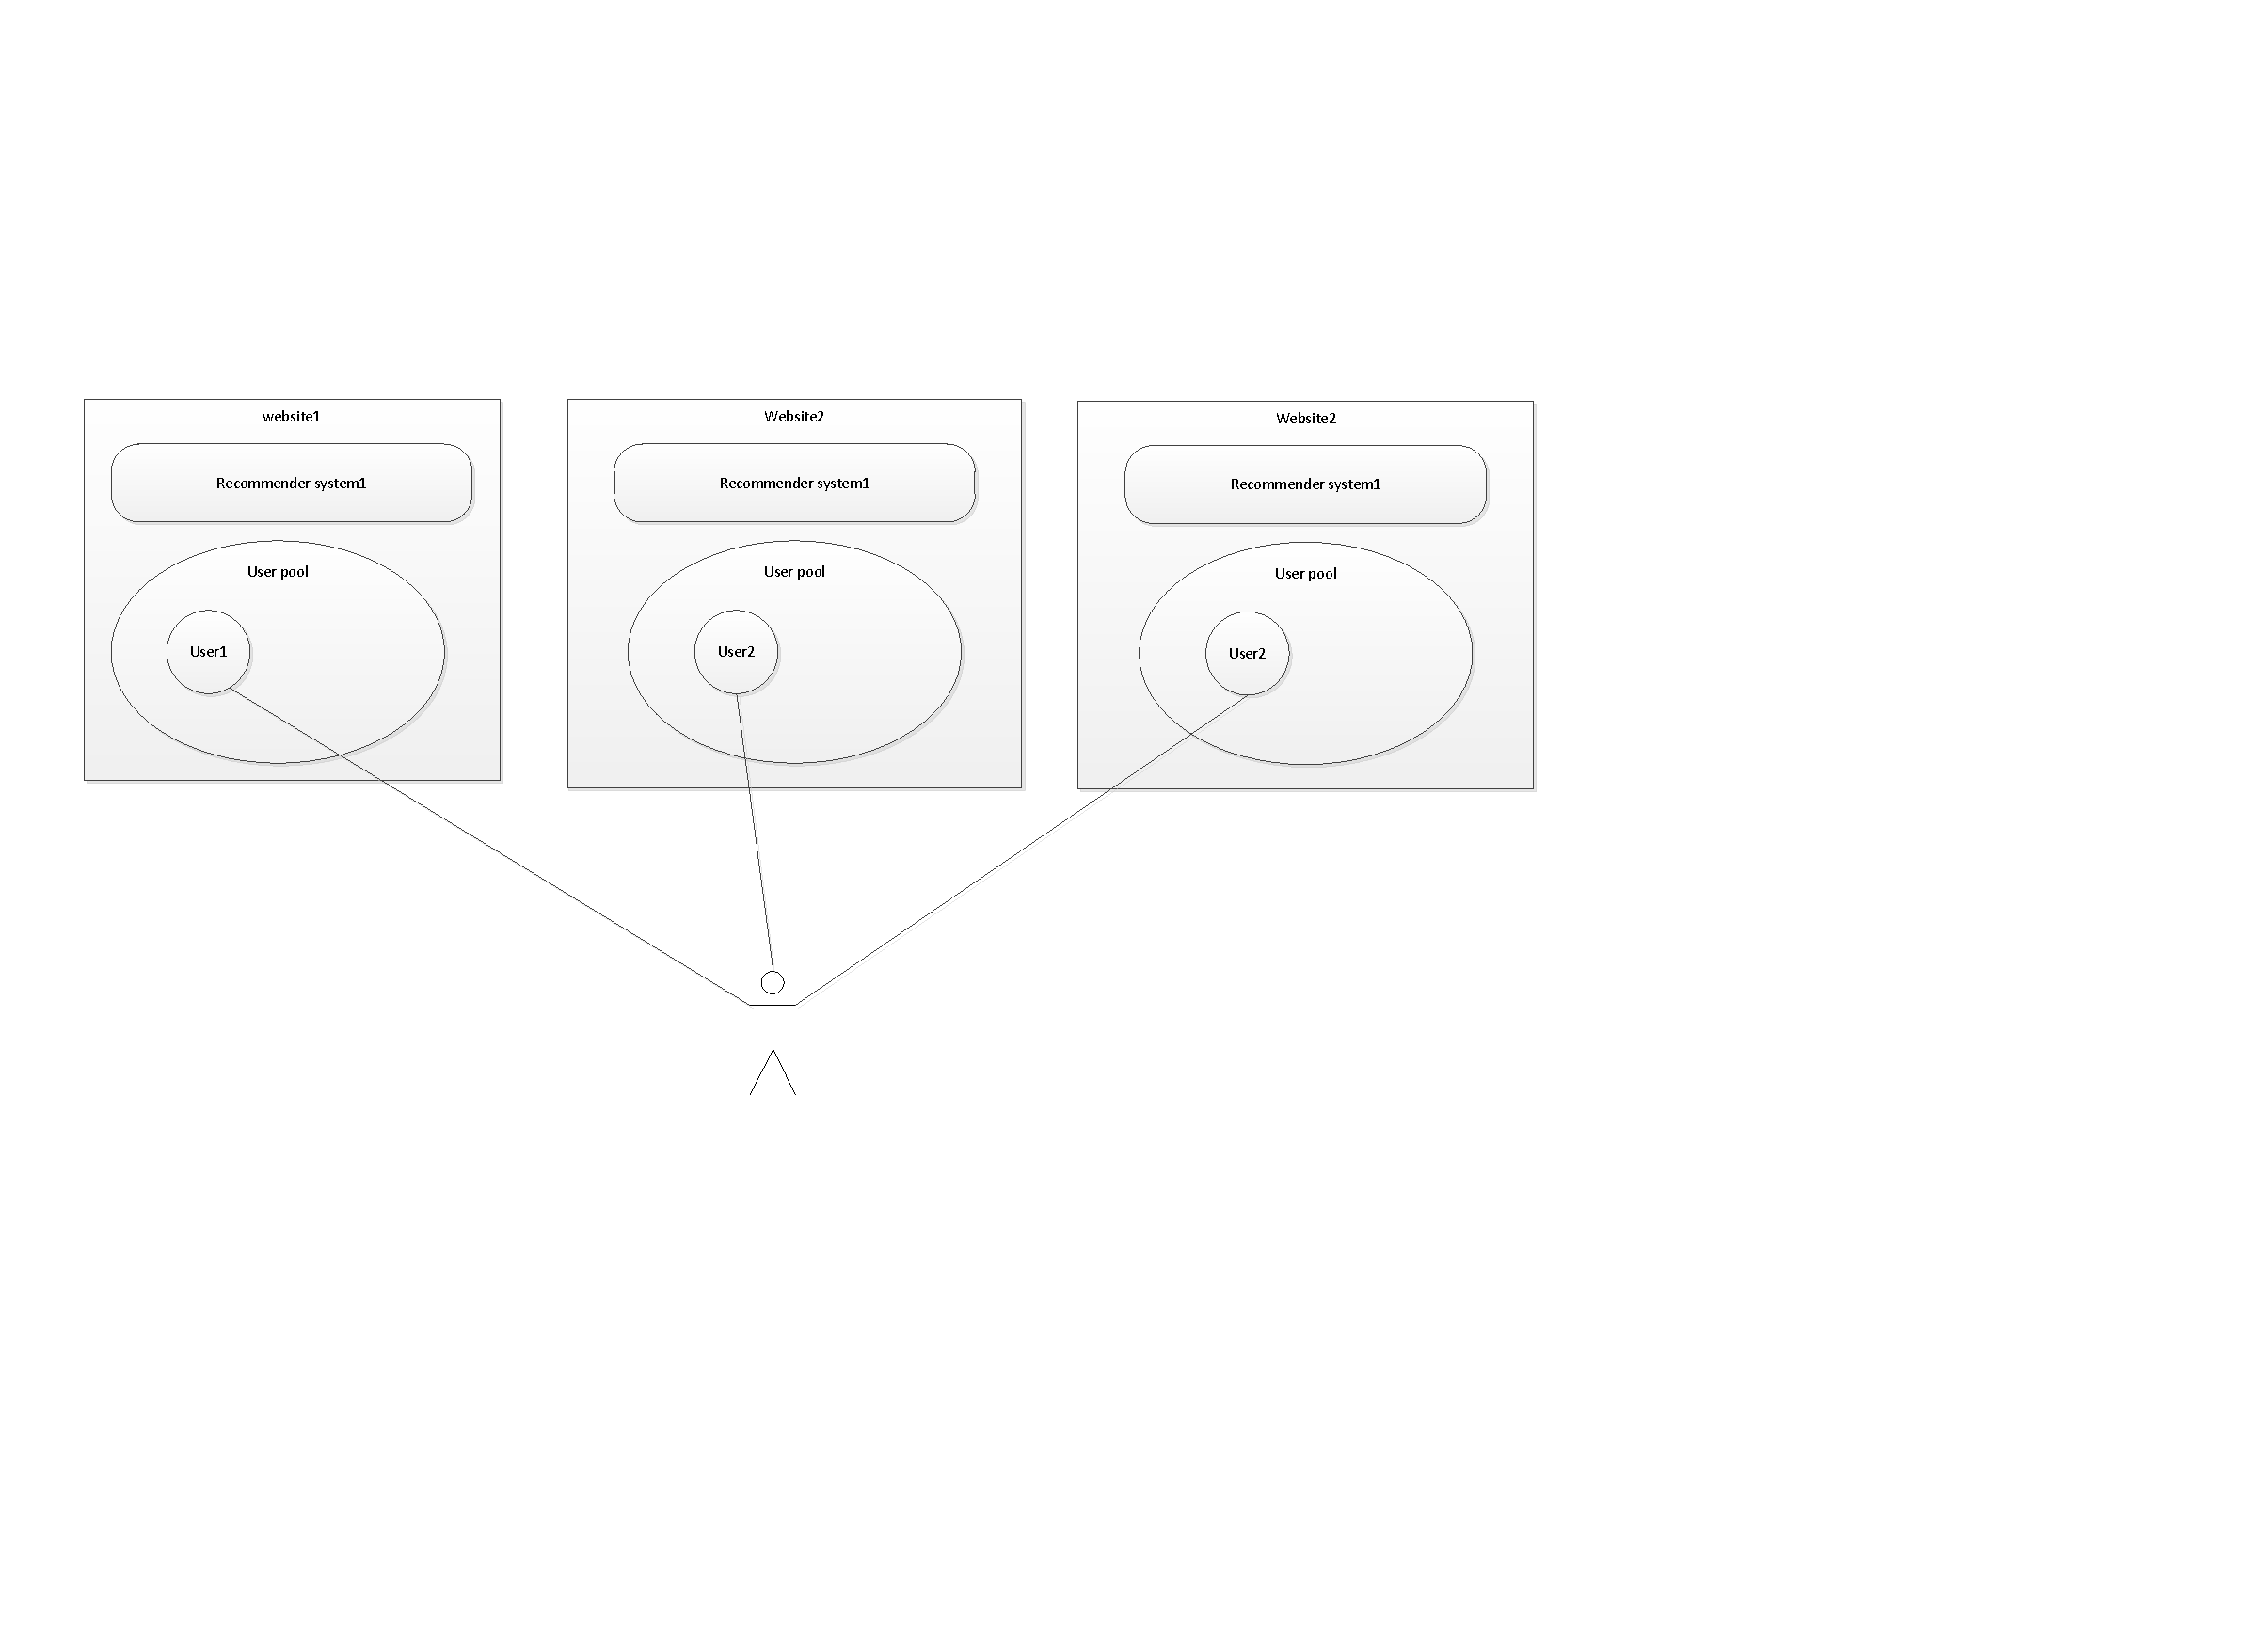
\includegraphics[width=\textwidth]{problem.pdf}
\caption{互联网平台的信息孤岛现象}
\label{fig:problem}
\end{figure}

举例来说,当用户作为信息获取者时,虽然每个网站可以为本平台上的用户提供很好的用户体验,通过数据挖掘等技术发现用户的兴趣,为其推荐有潜在需求的信息,但是不同网站之间的用户兴趣不能共享,导致兴趣推荐的不准确。当用户作为信息发布者时,其操作会更加繁琐,他往往需要打开多个网站重复几乎相同的操作来发布同样的内容,最明显的证据就是同时使用微信、微博和人人的用户需要在三个平台上重复三次操作完成发布。当这些网站越来越多的时候,问题也随之而来,即用户可能需要打开很多个独立的网站来完成一系列类似的事情。比如,先在新闻网站上浏览最新发生的时事,接着在摄影网站上发布新照片,然后在社交网站上浏览好友更新的状态,最后在电商网站上购买一些商品等等。换句话说,用户是单向地去寻找想要的信息,这其中无疑包含了一些不必要的重复操作。退一步来说,即使存在某些用户只在社交网站上浏览信息,很少接触其它网站,也会有一些重复操作的问题。因为该用户的好友很有可能是分散地活跃于各个不同的社交网站平台(微博、人人网等),而且每个平台发布的信息肯定有所不同,所以该用户仍然需要逐个登录各个网站后才能浏览到各个用户的信息。再退一步说,即便现在已经有些软件把所有社交网站整合成一个统一接口,让用户只需一次登录就能同时访问多个平台,用户仍然会遇到信息冗余的问题,比如重复的新闻、不感兴趣的推荐等等。

为了解决上述问题,现在设想有这样一个智能系统:每当用户打开系统时,系统会自动推送今天的时事新闻、其好友最近更新的状态、感兴趣或者正在促销的商品,以及一些根据用户偏好过滤的信息。此外,他也可以在系统上发布自己的信息给他的好友,甚至给那些对他信息感兴趣的陌生人。虽然,实现这样一个系统的工作量和难度是巨大的,但仔细观察后可以发现这样一个重要的规律:即用户希望所有的信息能够在整个互联网上智能地自主流动,在用户单方面寻找信息的同时,让信息也能自主地流向符合特定需求的用户。

\begin{figure}
\centering
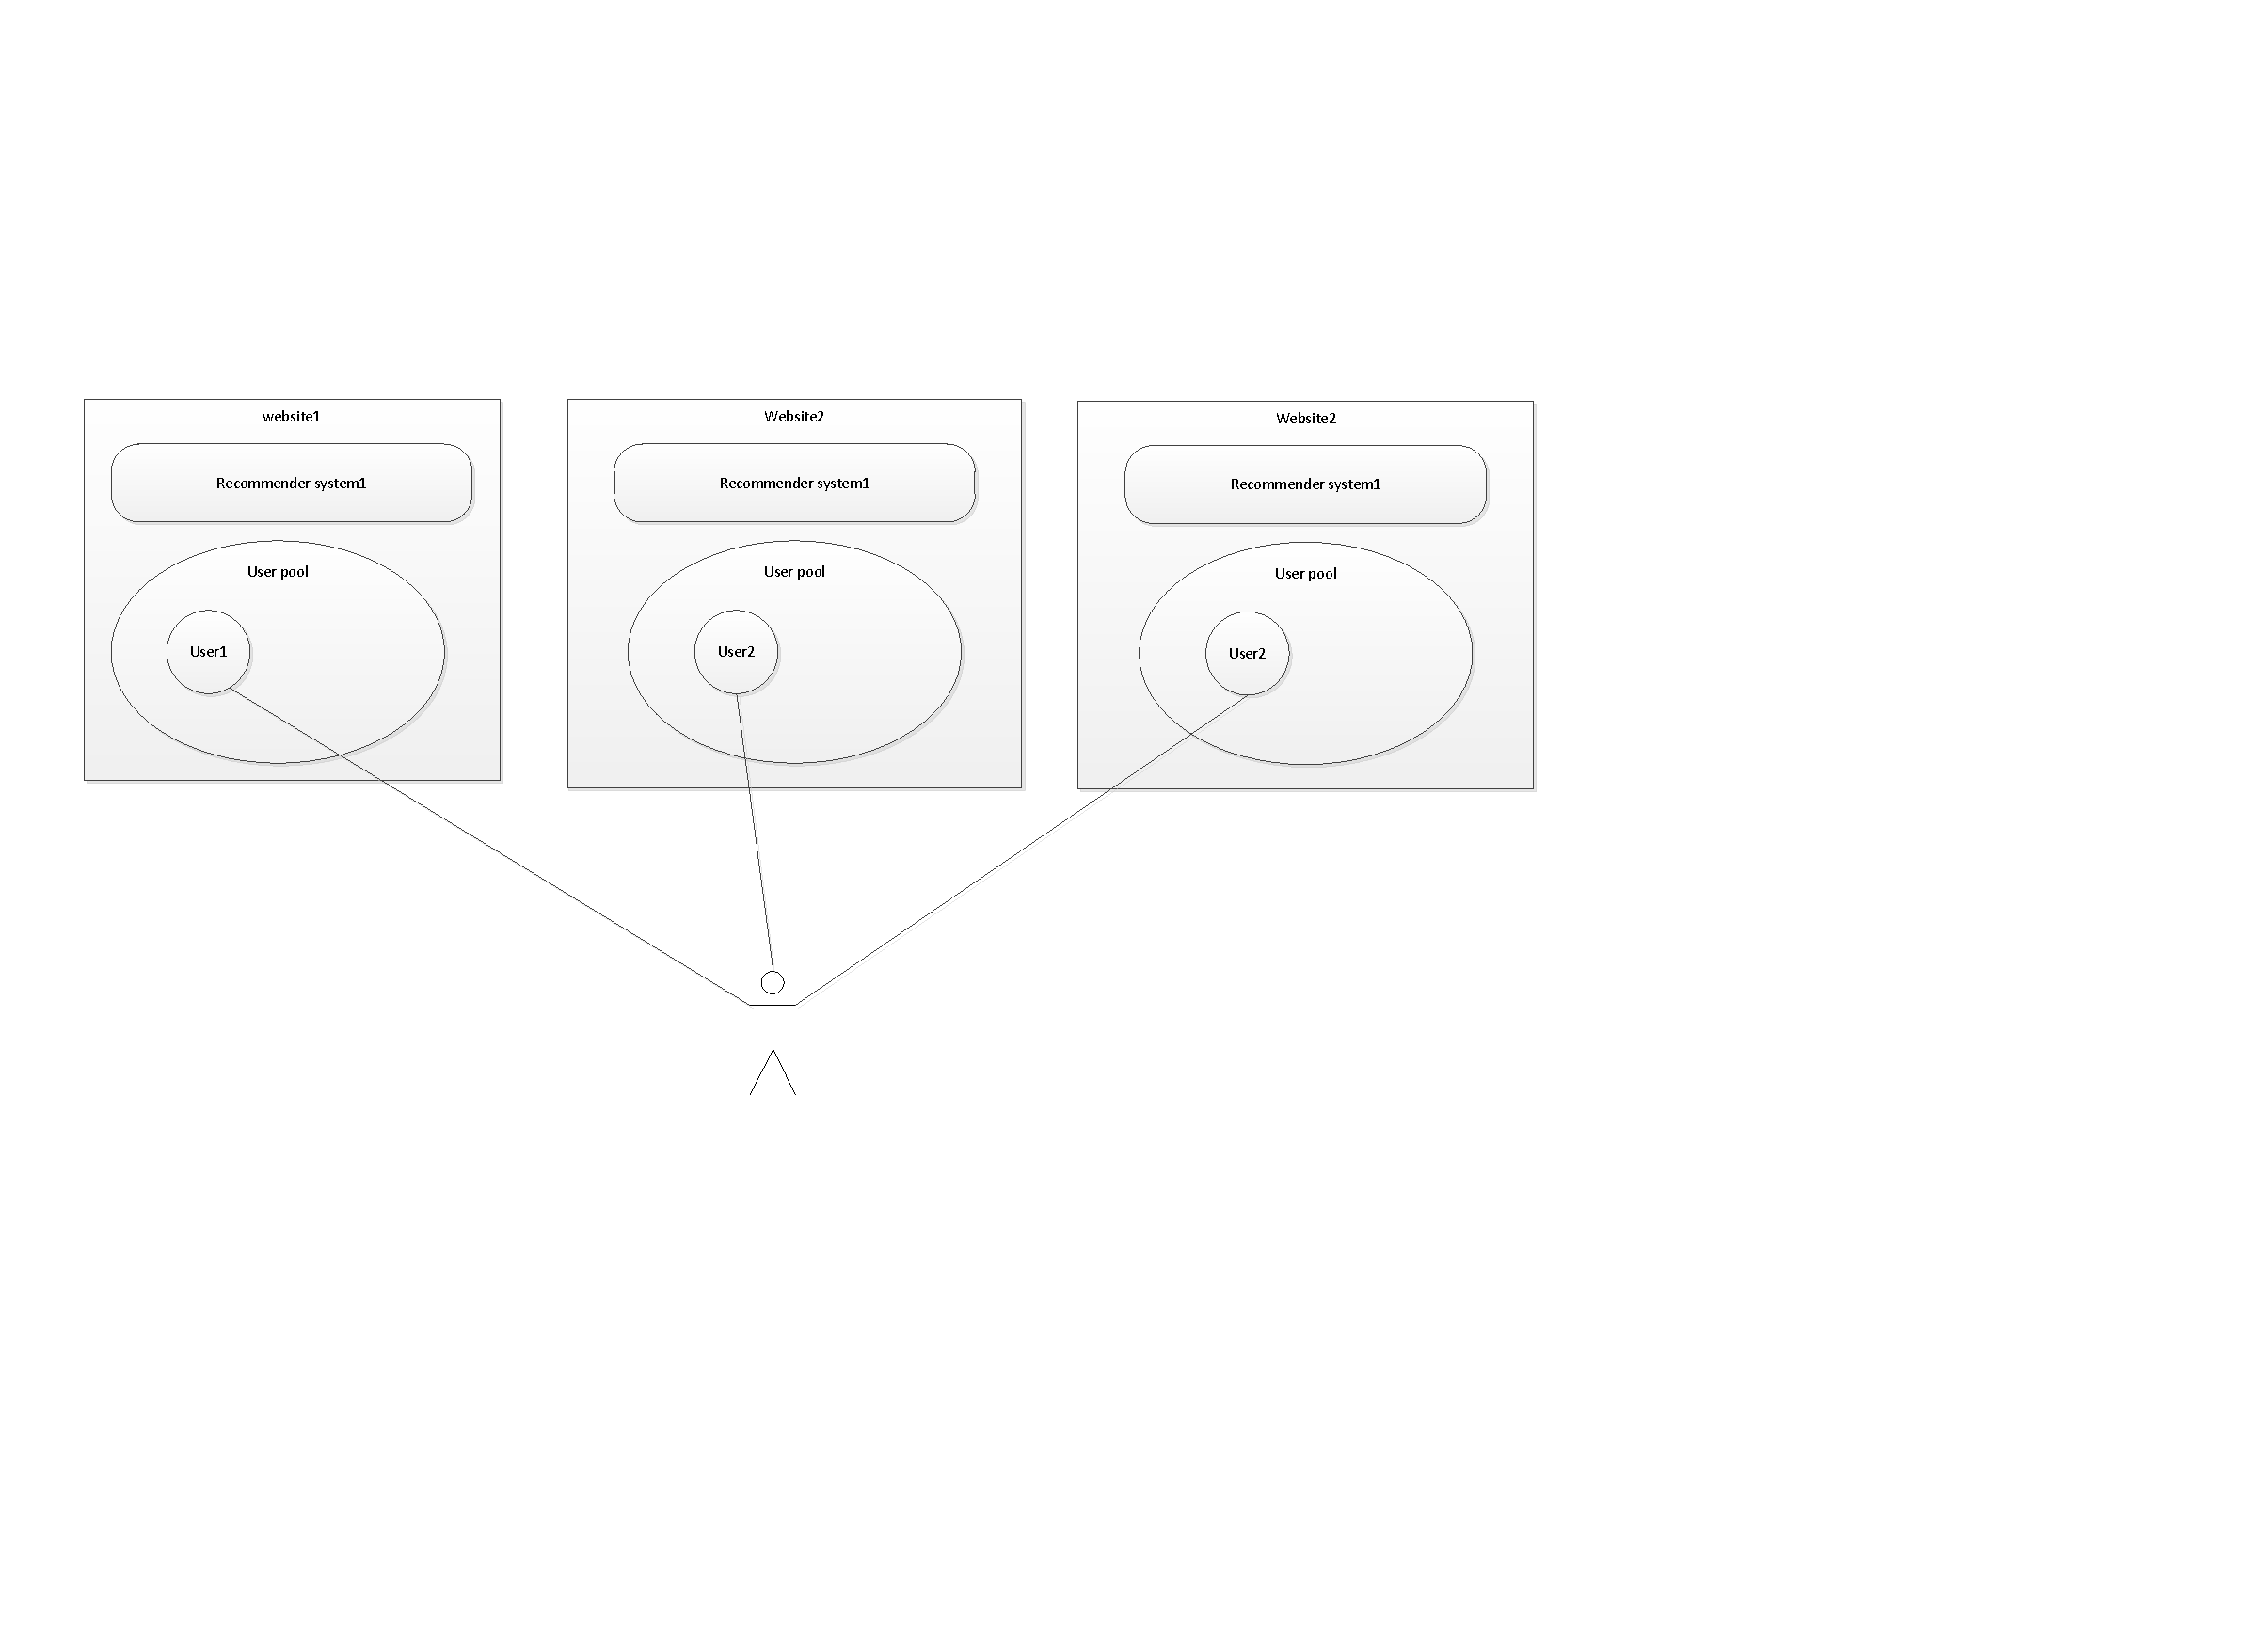
\includegraphics[width=\textwidth]{problem.pdf}
\caption{一种基于P2P网络的智能系统解决方案}
\label{fig:solution}
\end{figure}

从抽象层面来看,要实现这样一套信息自主流动的机制,传统的集中式计算模式已经不再适用。如图\ref{fig:solution}所示,这里每个用户均看作一个独立的节点,所有的节点整合在一起就形成一个巨大的P2P网络。其中,每个节点既充当服务器用于分发信息,也充当客户端用于接收信息,并且由某个节点发出的信息在其它节点间传播的时候会自主流动,寻找潜在的、匹配的节点。简单来说,要使信息能够自主流动,就要攻克这几方面的难点:

\begin{itemize}
\item 资源信息描述与匹配:互联网资源普遍呈现出半结构化或非结构化的特征,以普通的新闻或者博客为例,除了作者、标题、时间等结构化信息,正文纯文本都是典型的非结构数据。因此, 如何从这些非结构化的文本信息中提取出有用的特征、并用这些特征来衡量这些文本之间的相关性是本文重要研究内容。
\item 用户兴趣挖掘与关联:用户的兴趣可以从其发布和查看的信息中反映出来,基于上述对资源信息的描述模型,可以训练出某一时刻或者某一时段内的用户兴趣。但是,由于用户兴趣可能会随着时间的推移而不断变化,并且在同一时刻可能同时存在长期兴趣和短期兴趣。因此,这部分需要基于资源模型来解决用户兴趣随时间变化的问题。
\item P2P网络路由与搜索:从整个网络结构来看,在初始状态下各个用户节点之间的关系仅仅为物理意义上的距离关系,换句话说,节点与节点之间的边的权重不能代表用户与用户之间兴趣的相似度,从而也就导致每个节点上的信息不能自由传播。因此,这部分需要借助用户兴趣模型,通过P2P网络的路由搜索算法来寻找潜在的相似节点,最后构成某一时间段内的稳定结构。 
\end{itemize}

\subsection{研究意义与应用价值}
对于上述提出的信息孤岛现象是主要由目前网站之间相互独立而导致的,这些中心化结构的独立网站架构存在以下几个问题:

\begin{itemize}
\item 从资源传播的角度来看,每个网站的数据都仅仅在一个局部范围内可用,但是用户却要在多个这样的局部范围内同时使用多个网站。虽然对于每个网站可以维护相对较好的资源整合和管理,但是对于属于用户的资源的传播带来了很大的阻碍。
\item 从计算资源的角度来看,每个独立的传统B/S架构的网站通常由背后的一套计算群组来支撑,当网络流量十分巨大的时候,服务器的硬件和软件性能决定了系统平台可承受的最大程度。而在用户这边的客户端的I/O消耗相对小很多,但是大量客户端的请求对于服务器是一个不小的考验,从而导致了服务器成为整个系统的计算瓶颈。
\item 从隐私安全的角度来看,目前网站的数据均由平台自己的数据库进行维护,对于数据泄露成为重大隐患之一,即使网站的安全性是非出色,用户也会担心其数据是否会被第三方利用于商业用途。
\item 从拓扑架构的角度来看,用户与网站系统组成了中心化的拓扑结构,该结构不利之处在于当网站服务器宕机或者网络中断的时候,所有用户均无法访问该系统,这就使得网站系统的备份机制与主从切换机制十分完善,而对于大部分初创公司的流量有限和资金不足等特征是一个很大的考验。
\end{itemize}
  
与中心化结构网站架构不同,在基于P2P网络架构中,每个节点都可以既可以充当服务器为其它节点提供资源,也可以作为客户端向其它节点获取资源。综合来说,P2P网络的应用具有以下几大优点\cite{罗杰文2005peer}:

\begin{itemize}
\item 非中心化(Decentralization):在P2P网络中,节点之间的通信无需经过中心服务器,因此大大降低了服务器因为计算资源问题而导致的性能瓶颈。同时,网络中的信息资源完全存储在各个节点中,信息的交互完全在节点之间进行。
\item 可扩展性(Scalability):由于P2P网络中的每个节点可以看做服务提供者,所以每当有新的节点加入时,相当于扩充了整个网络的服务能力和资源,相反用户节点也可以随时退出,十分的灵活。以网络下载资源为例,普通C/S模式的计算下载通道的传输能力基本依赖于服务器的带宽,当用户一旦很多的时候,下载速度往往会受到很大的影响,但是在P2P网络中却恰恰相反,更多的节点请求意味着有更多的资源提供者,从而下载速度也更快。
\item 健壮性(Robustness):与中心化架构模式不同,P2P网络不会因为某一个节点退出而在很大程度上影响网络的正常运行,相反只有很小的一部分影响。结构良好的P2P网络一旦在某几个节点发生异常的时候会自动调整拓扑结构,从而保证整个网络的连通性。
\item 安全性(Security):传统集中式的计算模式在通信上往往需要经过中心服务器,也就是说用户的数据信息会全部经过这些服务器,因此只要在这些为数不多的服务器上动些手脚,用户隐私就会被泄露。但是,在P2P网络上则不同,信息传输不会经过某些特定的节点,并且还可以与特定有需求的目标节点建立连接,从而在很大程度上提升了匿名通信的可靠性以及灵活性。
\item 负载均衡(Load-Balance):根据上文所述,P2P网络下的用户节点既能充当信息发布者的角色,也可以作为信息接受者的角色,所以在计算资源和存储资源的分布十分均匀。同时,对于信息接受者来说,其可以向计算资源空闲的节点请求资源,而不用排队等待那些繁忙的节点直到任务完成。
\end{itemize}

基于上述有点,本文首先建立一套用于描述互联网信息和用户行为偏好的模型,旨在将这些具体的信息和用户行为偏好上升到抽象层面,剥离出一个统一的输入输出接口。对于那些专注于复杂的数据分析和建模工作的模块,该接口起到了整合的作用。而且,在此之后,也可以展开专门基于该描述模型的信息与用户匹配算法的研究。其次,根据上述信息描述模型与用户行为偏好模型的特点,从拓扑结构,通信机制等方面入手,建立一套合适的分布式架构(如P2P的计算模式),并利用上述的匹配算法,研究由各个节点组成的覆盖网络间的信息自主流动的机制。最后,将上述两项内容结合在一起,实现一套完整的信息自主流动的原型系统。

\subsection{国内外研究现状}
从目前的科学研究和商业应用方面来看,还没有关于一套基于P2P网络的信息自主流动机制的相关工作。因此,这部分将从文本信息挖掘、用户兴趣关联以及P2P网络搜索等三方面来具体展开阐明已有的研究工作。

\subsubsection{文本挖掘相关工作}
在文本信息挖掘方面,由于当今的硬件和软件技术在各方面都有大幅度提高,产生了大量的不同类型的数据资源\cite{han2006data},特别是纯文本的数据。这些文本大多来自于社交网络、新闻博客等网站,内容形式对于人们来说也是十分的丰富。但是这对机器来说却没有那么容易识别,因此需要设计一系列的算法来从这些文本数据中找出一些模式和规律,从而让机器更好地利用这些数据为人们创造更大的价值。结构化数据(Structured)通常可以存储在各类数据库中,但是纯文本数据却因为它的半结构化(Semi-structured)或者非结构化(Unstructured)特性从而只能有通过搜索引擎等技术才能进行索引和查找\cite{croft2010search}。搜索引擎是信息检索(IR)中的一种方式,其作用是方便用户直接通过输入关键词找到内容相关的文档集合,其目标是如何通过有效和高效的方法是检索的结果更加精确,涉及的研究领域包括文本聚类、文本分类、文本概括、推荐系统等\cite{grossman2004information,manning2008introduction,salton1983introduction}。但是,在本文中,除了这些信息检索基本的需求,更重要的是从文本中挖掘出重要的特征和模式,将原本非结构化的数据量化成半结构化数据,并且这种量化过程更多地从用户兴趣这点切入的。针对这个要点,文本挖掘技术一般可以分为以下几大类:

\paragraph{文本抽取}
文本抽取(Text Extraction)主要是从半结构化或结构化的纯文本里找出结构化信息,涉及了自然语言处理(NLP),信息检索和Web挖掘(Web Mining)等领域的技术。该研究最基本的两大工作是:a)命名实体检测(NER),包括找出文本中的人物、地点、组织等等;和b)关系抽取(Relation Extraction),主要包括名字之间的地理位置关系、人物关系、动作执行关系等等。

其中,对于命名实体检测问题,主要包括基于规则的方法\cite{appelt1993fastus,mooney1999relational}和基于统计学习的方法,后者有三个十分著名和常用的方法:隐马尔可夫模型(HMM)\cite{dugad1996tutorial},这是一个简单且有效的生成模型(Generative Model),最大熵马尔可夫模型(MEMM)\cite{berger1996maximum},这是一个判别模型(Discrimitive Model),适合于训练集十分充足的情况,因为它能给出一个更小的预测误差,以及条件随机场(CRF)\cite{lafferty2001conditional},该模型是一个基于无向图的判别模型,因此适用于当前状态均受前后影响的情况。

对于关系抽取问题,主要包括基于分类的方法(Classification-based)\cite{kambhatla2004combining,guodong2005exploring,jiang2007systematic,chan2010exploiting}和基于核的方法(Kernal-based)\cite{bunescu2005shortest,zhao2005extracting}。其中,分类方法在应用之前需要对文本进行特征提取(Feature Extraction),比较有用的特征包括实体、词汇、语法和背景知识等。而核方法最常见的场景是先将文本用向量空间模型(VSM),再进行下一步计算,主要分为基于序列的核方法、基于树的和方法和混合核方法,在机器学习中,核函数(Kernal Function)是两组向量空间的内积,也可以看做观测值之间的一种相似度衡量方法,从而观测值不需要显示地映射成向量空间。

总结来说,当前命名实体检测最有效的方法都是基于概率图模型而提出的,典型代表是MEMM和CRF,而关系抽取的方法则是很大程度上基于选取的特征或者定义的核函数,然后再利用分类算法进行解决。可以发现,上述这些主流方法都是有监督方法,但是,随着互联网产生数据的规模不断增大,半监督和无监督方法会更加实用。

\paragraph{文本摘要}
文本摘要(Text Summarization)用于从纯文本中识别出重要的内容,包括重要的句子、关键词和主题等。因此根据不同的表示方式,基本方法可以分为主题表示法、标识符表示法、句子表示法。

其中,主题表示法需要首先找出一种主题描述的方式,一般是用主题词,这种词的特性是排除文档中出现频率高以及极少出现的词,然后利用对数似然比检验(LR Test)来识别那些能够很具有代表性的单词\cite{dunning1993accurate}。关于单词出现频率的计算方式,最经典的就是TF-IDF\cite{gupta2007measuring},这种方法一方面计算了单词出现的频率,另一方面也衡量了单词的重要性。再进一步,文献\cite{deerwester1990indexing}提出的潜语义分析(LSA)方法则用一种隐含的方式来表示文本中的语义信息,其十分适用于对新闻文本的总结,而且不需要使用第三方的词典数据就能实现。在LSA的基础上,更多的基于贝叶斯理论的主题模型被陆续提出,这些模型在主题表示上十分成熟,而且很多已经在工业界广泛使用\cite{daume2006bayesian,haghighi2009exploring,wang2009multi,celikyilmaz2010hybrid}。

对于句子粒度的摘要方法,通常是先将相似的句子进行聚类\cite{mckeown1999towards,hatzivassiloglou2001simfinder},其中相似度的计算方式包括简单的余弦相似度(Cosine Similarity)等。处于同一类中的句子被认为是某种主题,而有很多句子的类则说明包含了重要的主题,然后从每个这样的类中选取一个句子作为这种主题的代表,组合起来就是对文章的摘要。同时,对于选出来的句子可以用KL散度(KL Divergence)来进行评分,从而来判断选出来的摘要的好坏。

\paragraph{文本降维}
文本降维(Dimensionality Reduction)用于解决文本向量的维度过大的问题,这里主要的方法包括诸如LSI(Latent Semantic Indexing)、PLSI(Probabilistic Latent Semantic Indexing)和LDA(Latent Dirichlet Allocation)\cite{blei2003latent,heinrich2005parameter}等主题模型,这些模型共同的假设前提是把文档看做词袋模型(Bag-of-words),即不关心单词的先后顺序,从而可以更有效更快速地来处理文本。

对于主题模型来说,在整个文档集合$D$中,共有$M$篇文档,词汇表共有$W$个不同的词汇,并且假设总共有$K$个主题,其中文档和词汇都是已知的,主题为待求的问题。因为已经存在$D*W$维的文档-词汇矩阵$X$,通过主题模型以后本质是将该矩阵分解成两个矩阵:$D*K$维的文档-主题矩阵$A$,和$K*W$维的主题-词汇矩阵$B$,即$X=A*B$。在矩阵$X$中,每一行表示一篇文章$d_m$,每一列表示一个词汇$v_i$,每个值$x_{m,i}$表示该文档具有该词汇的比重,这个比重可以是通过正规化后的词频,也可以是TF-IDF的值。在矩阵$A$中,每一行表示文档$d_m$,每一列表示主题$z_k$,每个值$a_{m,k}$表示该文档具有该主题特征的权重,所以文档可以表示为一个关于主题的$K$维向量,从而将文档看成一个服从多项分布的随机变量$\vec{\theta_m}$。在矩阵$C$中,每一行表示主题$z_k$,每一列表示词汇$v_i$,每个值$b_{k,i}$表示该主题中该词汇占有的比重,由此可见,这里的每个主题表示为关于词汇的一个$W$维向量,从而主题可以看做一个服从多项分布的随机变量$\vec{\phi_k}$。关于如何求出参数$\vec{\theta_m}$和$\vec{\phi_k}$将在后文结合本文提出的模型具体详解。

但是诸如LDA这类的主题模型还有很多局限性,第一,LDA推理的方法大致分为两种Collapsed Gibbs sampling\cite{heinrich2005parameter}和Variational Approximation\cite{blei2003latent},但是两者在整个迭代过程中十分耗时,当数据量很大的时候,特别是词汇表的大小$W$达到百万级的时候,$\vec{\phi_k}$的维度十分高,导致计算很慢。因此,基于这个问题,目前已经提出了并行的亦或是分布式的LDA算法\cite{asuncion2009smoothing,smola2010architecture},从而应对工业界大规模数据的问题。第二,当文档集随时间变化时,LDA本身并不能很好适应这个动态的过程,一种方法是引入时间变量重构概率图模型。文献\cite{deerwester1990indexing}通过扩展了时间维度和LSI的张量分析从而实现了对历史文档的更新。文献\cite{varadarajan2010probabilistic,molgaard2009temporal}则在PLSI的基础上加上时间维度提出两个全新的主题模型,分别在视频中活动抽取和音乐抽取方面有所作为。David Blei作为LDA的提出者,后来根据时间动态变化这个需求又提出了基于时间演化的主题模型\cite{blei2006dynamic},很好地解决了这方面的问题。第三,有些文档间会存在关联,比如学术论文间可以以作者和引用上建立连接,在诸多改进方案之中,RTM模型(Relational Topic Model)\cite{chang2009relational}在LDA的基础上联合模拟文档和链接的生成过程,从而很好地解决了文档网络的问题。

总结来说,基于概率图的主题模型是一种很好的文本降维方式,一方面它以统计学中的降维方法为基础,使得可以推理或近似得出隐藏在文档背后的主题是什么,另一方面,它也给出了对主题的一种新的定义,并且基于这种定义使得模型能够很容易地根据不同类型文档的需求来改进。但是一个很重要的问题是如何能够将这些主题模型应用到实际工业界中,因为在性能、效率方面还是有不尽如人意的地方。

\subsubsection{用户兴趣挖掘相关工作}
用户兴趣偏好主要体现在其对文本资源的喜好程度,换句话说,对用户兴趣挖掘的过程类似于对文本挖掘的过程,但是在技术上有所不同。对于用户兴趣的分析主要包括三个方面:用户兴趣的描述方式、用户兴趣挖掘和用户兴趣的匹配。

\paragraph{用户兴趣描述}
传统的用户兴趣表示方法包括VSM\cite{gong2012personalized}、兴趣树等层次结构\cite{kim2003learning}以及基于本体构建的描述方式。其中,VSM是最基本的描述方式,即将用户的兴趣表示成一个向量,每个值表示用户对该兴趣的喜好程度。对于层次结构的兴趣,主要考虑了兴趣之间的相关性问题,以及兴趣概念的大小范围之分。而最近本体工程的发展使得很多研究都偏向于将用户兴趣基于本体进行构建。User Profile(UP)是一种表示用户信息的概念模型,由用户的背景知识生成而得,文献\cite{li2006mining,tao2011personalized}中提出UP作为描述用户偏好和行为的信息。比如在用户读文章的时候,就可以用这个概念模型来判断该文档是否符合该用户的口味。为了模拟用户的这种概念模型,可以使用本体(Ontology),即所谓的Ontological User Profiles\cite{pretschner1999ontology,sieg2007web},或者Personalized Ontology\cite{tao2007ontology},在文献\cite{trajkova2004improving}中提出了一种改进后的 Ontological User Profile。UP可以分为三大类:a)interviewing模式是最好的UP,因为它们通过人工的方式来获得的,比如通过问卷调查来分析用户所在的分组,一个典型的例子是TREC Filtering Track训练数据集,它就是纯手工采集的数据:受访者在读完某篇调查材料后会给出一个支持或反对的表态,由于只有用户最知道自己的兴趣所在,所以这些答案能十分精确地反映用户背景知识。b)Semi-interviewing则使用半自动技术来获得用户的信息,该技术往往是提供用户一系列分类列表,并要求用户选择自己喜欢的分类。c)Noninterviewing则完全不用让用户参与进来,而是观察用户的活动、行为以及背景知识。 一个典型的模型是OBIWAN,其通过用户浏览的历史记录来获得用户偏好。如图\ref{userprofile}所示,这是 一种基于若干种上述方法采集数据后建立的UP模型\cite{sieg2007learning}。

\begin{figure}
\centering
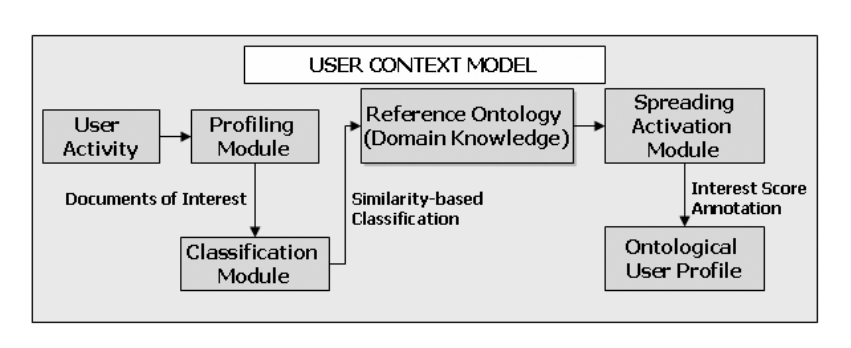
\includegraphics[width=\textwidth]{userprofile.png}
\caption{一种基于Ontological User Profile的环境模型}
\label{fig:useprofile}
\end{figure}

\paragraph{用户兴趣挖掘}
用户兴趣挖掘技术与文本挖掘类似,但是目的是不一样的。在情感分析(Sentimental Analysis)方面,可以使用常见的有监督分类算法对文本进行分类,比如朴素贝叶斯分类器(Naive Bayesian)和支持向量机(SVM),对用户正负情感进行分类\cite{pang2008opinion},当用户对某个文本资源产生负情感时,很有可能说明他对主题的资源没有兴趣,反之亦然。但是,在分类之前的特征选取有所不同,因为文档中表示情感的词的权重和否定词必须更大,而为了找出那些是具有主观色彩的词汇,又需要借助已经准备好的情感关键词字典等数据集。同理,对于无监督聚类算法也是适用的,并且反而更加接近真实状态\cite{taboada2011lexicon,taboada2007thumbs}。如果将分析的粒度从文档缩小到句子,也就是主观性分类问题(Subjectivity Classification),一些已有的工作\cite{riloff2006feature, riloff2003learning, wiebe2004learning, wilson2006recognizing}在这方面已经表现得十分出色,但是这些工作有一个假设前提,即假每个用户只会对一个句子产生一种情感。另外,单纯地从比较两个情感词不一定能够找出他们之间的关系,这时候依然需要借助于情感字典\cite{miller1990introduction},即事先定义好近义词、反义词、上义词和下义词等等,这样就可以匹配两个含义类似但拼写或者写法完全不同的两个词。

\paragraph{用户兴趣匹配}
用户兴趣的匹配主要体现在为兴趣类似的用户推荐资源,在各大电子商务平台中都存在着这样的推荐系统,其背后的原理就是基本的协同过滤算法(Collaborative Filtering)\cite{su2009survey,shi2014collaborative}。CF是在信息过滤和信息系统中正迅速成为一项很受欢迎的技术。与传统的基于内容过滤直接分析内容进行推荐不同,协同过滤分析用户兴趣,在用户群中找到指定用户的相似(兴趣)用户,综合这些相似用户对某一信息的评价,形成系统对该指定用户对此信息的喜好程度预测。典型的协同过滤推荐算法是基于用户的协同过滤推荐算法,其基本原理是利用历史评分数据形成用户邻居,根据评分相似的最近邻居的评分数据向目标用户产生推荐。基于用户的协同过滤推荐是基于这样一个假设:如果用户对一些项目的评分比较相似,则他们对其他项目的评分也比较相似。推荐过程可分为三步:a)首先获得用户对项目的评分,建立用户一项目评分矩阵;b)计算目标用户与其他各个用户的相似度,得到目标用户的最近邻居集合;c)根据其最近邻居对项目的评分信息预测目标用户对未评分项目的评分,取出预测评分最高的前n项推荐给用户,完成推荐。如图\ref{fig:cfsurvey}所示,CF主要分为三大类,即基于记忆的CF、基于模型的CF和混合CF。其中,基于记忆的CF通常使用用户对资源的评价信息来计算用户之间的兴趣相似度,再根据相似度来给出推荐和预测。该方法的不足之处是由于用户评价过的资源数量相对于资源总数是一个很小的值,导致了数据十分稀疏,从而推荐不准确甚至无法推荐。基于模型的CF则直接使用评价的数据来训练模型,并用过模型来做预测,这些模型包括上面提到的主题模型、聚类算法等,但是这些模型本身的缺陷会在CF预测的过程中带来潜在影响。混合Cf则结合上述两种方法,在一定程度上可以弥补上述方法各自的缺陷。

\begin{figure}
\centering
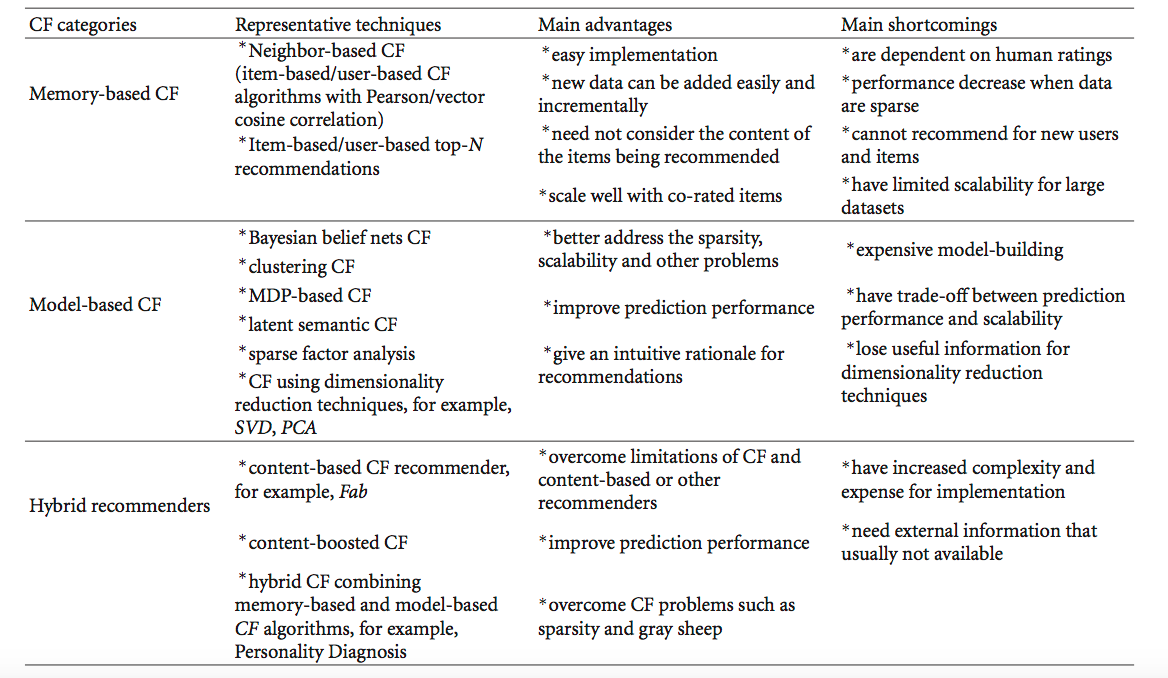
\includegraphics[width=\textwidth]{cfsurvey.png}
\caption{协同过滤推荐算法的综述}
\label{fig:cfsurvey}
\end{figure}

\subsubsection{P2P网络路由搜索相关工作}
P2P网络主要以其非中心化特点为主,因此主要研究问题集中在网络中的搜索技术,但是搜索的方法在很大程度上基于整个网络的拓扑结构,因此下面从拓扑结构和搜索技术两部分来阐述现有工作。

\paragraph{P2P网络的拓扑结构}
拓扑结构表示P2P网络中各个节点之间在物理或者逻辑上相互连接的关系,主要有四种类型:中心化拓扑、全分布式非结构化拓扑、全分布式结构化拓扑、半分布式拓扑。这四类拓扑结构的优缺点比较如图\ref{tbl:topologycomp}所示。

其中,中心化拓扑结构最为简单,典型的例子是Napster\footnote{http://www.napster.com/},该结构与传统的中心化服务器架构类似,普通的节点需要从中央索引服务器中获取其他节点的信息,从而才能进行路由,该结构的好处是十分便于节点搜索复杂的内容,并且速度十分快。但是,该结构的缺陷也十分明显,一旦中央索引服务器宕机时,整个网络就会处于瘫痪状态,因此该拓扑不适用于大型的网络系统。全分布式非结构化拓扑适用于覆盖网络(Overlay Network),该结构一般基于随机图来构建,节点的度数服从幂定律(Power-Law)\cite{ripeanu2002mapping},因为节点之间没有严格定义的关系,所以该拓扑具有很好的灵活性,动态变化的结构在容错计算上也有很好表现,经典的案例是Gnutella\cite{ripeanu2001peer}。但是,由于该拓扑结构是完全随机的,因此具有一定的不可预见性,在查找和搜索方面也相对复杂很多。全分布式结构化拓扑则是一种综合了上述两种拓扑的特性,使用了分布式散列表(DHT)来组织网络中的节点关系,典型的例子包括Tapestry\cite{zhao2001tapestry}、Pastry\cite{rowstron2001pastry}和Chord\cite{stoica2001chord}等等。DHT的作用是将网络中节点的名字映射到散列表中,这样可以更加快速地进行查找,而且同时也支持动态添加和删除节点。半分布式拓扑(Hybrid Structure)则是一种介于中心化结构和完全分布式结构之间的一种拓扑,在网络中存在一些超级节点(Super Node/Hub),这些节点与中心化拓扑中的中央索引服务器作用类似,提供周围节点的信息。当有源节点提出请求时,这些超级节点会互相通信,找出目标节点的位置等相关信息,并返回给源节点以供其进行连接,一个著名的例子就是KaZaa\cite{good2003usability}。

\begin{table}
\caption{P2P网络四种拓扑结构的优缺点对比(A最好,D最差)}
\centering
\begin{tabular}{|c|c|c|c|c|} 
\hline
拓扑 & 中心化 & 全分布式非结构化 & 全分布式结构化 & 半分布式 \\
\hline
可扩展性 & D & D & B & C \\
\hline
可靠性 & D & B & B & C \\
\hline
可维护性 & A & A & B & C \\
\hline
搜索性能 & A & C & B & B \\
\hline
复杂查询 & 支持 & 支持 & 不支持 & 支持 \\
\hline
\end{tabular}
\label{tbl:topologycomp}
\end{table}

\paragraph{P2P网络的搜索技术}
P2P网络中由于每个节点仅仅存储有限的信息,包括节点本身的网络配置、索引服务器的信息以及周围小部分节点的信息等,因此需要通过搜索算法来找到要与之建立连接的目标节点。在结构化拓扑的P2P网络中,搜索算法常常是基于DHT查找就能完成。在非结构化拓扑的P2P网络中,搜索算法都是基于小世界理论\cite{watts1998collective},常见的搜索算法有以下几个\cite{tsoumakos2006analysis}:

\begin{itemize}
\item Flood Fill:这个算法最早用在Gnutella协议中,与传统的图算法BFS类似,即先搜索当前节点的所有邻居节点,然后对每个邻居节点执行相同的操作。该方法实现起来十分简单,但是会产生大量的网络流量并造成网络拥堵。
\item Modified-BFS:该方法在Flood Fill的基础上加上一个概率条件,即以一定的概率选取部分邻居节点,其他不变。
\item Iterative Deepening:该方法是在Flood Fill的基础上增加了一个阈值TTL(Time to Live),从而控制了搜索半径。
\item Random Walk:这个算法基于图的DFS搜索,首先随机选取源节点的一个邻居节点,并对该邻居节点进行同样操作,直至完成一条完整路径的索索,然后从源节点开始重新执行这些操作\cite{bisnik2005modeling}。
\item Agent-based:移动Agent是一个在网络中交换和传递资源的程序,也就是所有的搜索的任务都有网络中的agent来完成,agent与agent之间也会交换信息,从而实现搜索\cite{babaoglu2002anthill}。
\item Query Routing:这个方法是直接对每个节点的资源建立索引,同时也会记录周围节点的索引信息,所以当查询请求来到时,不用再次转发给其他节点进行搜索,而是直接从索引表中定位到目标资源的位置信息,并直接与目标节点建立连接。
\end{itemize}

总结来说,这些方法在一定程度上已经十分适应很多分布式的场景,但是随着移动设备的普及,每个移动设备可能也是一个潜在的节点,但是这些设备的加入或退出更大地加剧了网络波动(Churn),从而导致整个网络拓扑结构的不稳定,并且如何保证在这种大波动的情况下进行精确的查询和搜索是未来P2P网络中搜索技术的一大挑战。

\subsection{本文内容安排}
本文的主要内容安排如下。首先本章对该研究的背景,主要研究内容和研究意义与研究现状进行了一个总体的介绍。第二章将对基于P2P网络的信息自主流动机制提出一个完整的技术方案,并且结合研究现状和存在的问题对设计需求和挑战进行详细描述,从而给出关键的技术点。第三章将对解决方案中的第一部分即文本资源的描述与匹配问题进行深入分析,通过结合现有成熟的模型,提出一整套全面的理论模型。第四章将结合第三章的研究基础对用户兴趣进行建模,结合现实中兴趣的动态变化特征给出相应的解决方案。第五章将基于第四章的研究基础提出一种基于P2P网络的路由与搜索算法,从而实现动态构建兴趣覆盖网络。第六章将根据第三、四、五章的理论进行模拟实验和真实实验,验证上面提出的新的方法的有效性。第七章则基于前文的研究成果实现了一套简单的智能系统原型,包括功能设计和系统架构等方面。最后第八章对本研究做了一个总结,并对研究进一步的工作方向进行了讨论。

